\documentclass[border=10pt]{standalone}
\usepackage[T1]{fontenc}
\usepackage{helvet}
\renewcommand{\familydefault}{\sfdefault}
\usepackage{tikz}
\usetikzlibrary{arrows.meta,positioning,calc,shapes.geometric}

\definecolor{idpblue}{HTML}{005DAA}
\definecolor{idpcyan}{HTML}{00B3FF}
\definecolor{warm}{HTML}{D7263D}
\definecolor{inkgray}{HTML}{444444}
\definecolor{forestgreen}{HTML}{2E7D32}

\begin{document}
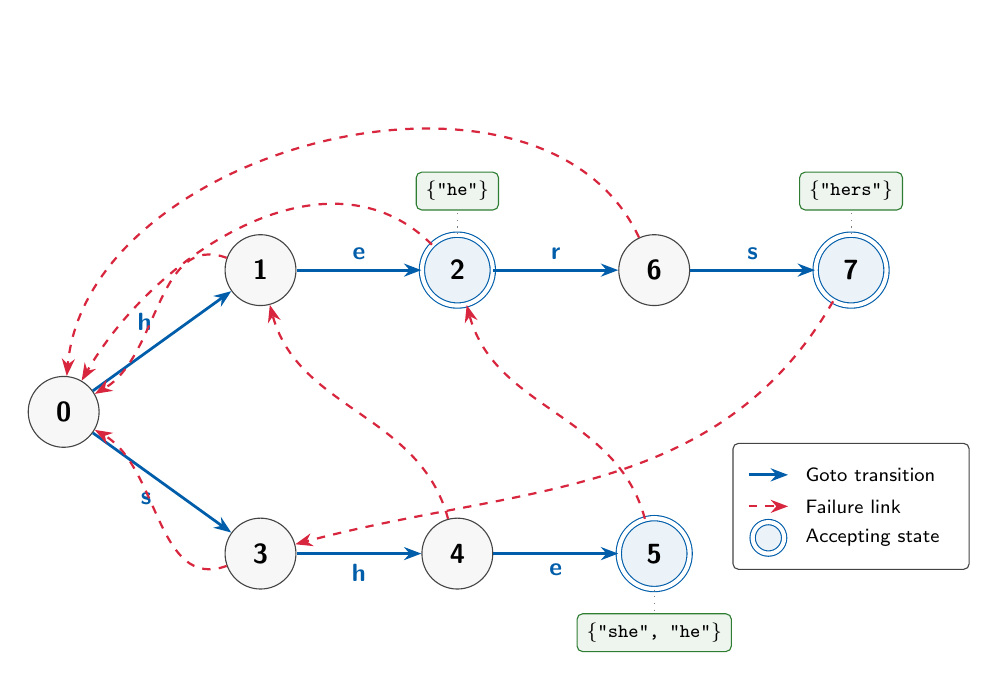
\begin{tikzpicture}[
    font=\small,
    >={Stealth[length=2.2mm]},
    state/.style={draw=inkgray, circle, minimum size=9mm, fill=gray!6, font=\bfseries},
    accept/.style={state, double, double distance=1.5pt, draw=idpblue, fill=idpblue!8},
    goto/.style={->, line width=1.0pt, idpblue},
    fail/.style={->, dashed, line width=0.8pt, warm},
    match/.style={draw=forestgreen, rounded corners=2pt, fill=forestgreen!8, font=\scriptsize\ttfamily, align=center},
]

    % --- Nodes ---
    \node[state] (s0) at (0, 0) {0};
    
    % Upper branch (h -> he -> her -> hers)
    \node[state] (s1) at (2.5, 1.8) {1};
    \node[accept] (s2) at (5.0, 1.8) {2};
    \node[state] (s6) at (7.5, 1.8) {6};
    \node[accept] (s7) at (10.0, 1.8) {7};
    
    % Lower branch (s -> sh -> she)
    \node[state] (s3) at (2.5, -1.8) {3};
    \node[state] (s4) at (5.0, -1.8) {4};
    \node[accept] (s5) at (7.5, -1.8) {5};

    % --- Match Labels ---
    \node[match, above=3mm of s2] (m2) {\{"he"\}};
    \node[match, below=3mm of s5] (m5) {\{"she", "he"\}};
    \node[match, above=3mm of s7] (m7) {\{"hers"\}};

    % Connect labels to states
    \draw[gray, thin, dotted] (s2) -- (m2);
    \draw[gray, thin, dotted] (s5) -- (m5);
    \draw[gray, thin, dotted] (s7) -- (m7);

    % --- Goto Transitions ---
    \draw[goto] (s0) -- (s1) node[midway, above left, font=\small\bfseries] {h};
    \draw[goto] (s1) -- (s2) node[midway, above, font=\small\bfseries] {e};
    \draw[goto] (s2) -- (s6) node[midway, above, font=\small\bfseries] {r};
    \draw[goto] (s6) -- (s7) node[midway, above, font=\small\bfseries] {s};
    
    \draw[goto] (s0) -- (s3) node[midway, below left, font=\small\bfseries] {s};
    \draw[goto] (s3) -- (s4) node[midway, below, font=\small\bfseries] {h};
    \draw[goto] (s4) -- (s5) node[midway, below, font=\small\bfseries] {e};

    % --- Failure Transitions ---
    % f(1) = 0
    \draw[fail] (s1) to[out=160, in=30] (s0);
    
    % f(2) = 0
    \draw[fail] (s2) to[out=135, in=60] (s0);
    
    % f(3) = 0
    \draw[fail] (s3) to[out=-160, in=-30] (s0);
    
    % f(4) = 1
    \draw[fail] (s4) to[out=105, in=-75] (s1);
    
    % f(5) = 2
    \draw[fail] (s5) to[out=105, in=-75] (s2);
    
    % f(6) = 0
    \draw[fail] (s6) to[out=115, in=85] (s0);
    
    % f(7) = 3
    \draw[fail] (s7) to[out=-120, in=15] (s3);

    % --- Legend ---
    \begin{scope}[shift={(8.5, -1.8)}]
        \draw[inkgray, fill=white, rounded corners=2pt] (0, -0.2) rectangle (3.0, 1.4);
        
        \draw[goto] (0.2, 1.0) -- (0.7, 1.0);
        \node[anchor=west, font=\scriptsize] at (0.8, 1.0) {Goto transition};
        
        \draw[fail] (0.2, 0.6) -- (0.7, 0.6);
        \node[anchor=west, font=\scriptsize] at (0.8, 0.6) {Failure link};
        
        \node[accept, minimum size=4mm] at (0.45, 0.2) {};
        \node[anchor=west, font=\scriptsize] at (0.8, 0.2) {Accepting state};
    \end{scope}

\end{tikzpicture}
\end{document}
